\documentclass[10pt,twocolumn]{article}
	
\usepackage{myfontstyle}
\usepackage{mypackages}
\usepackage{mymacros}
\usepackage{mycommands}
\usepackage{graphicx}
\usepackage{hyperref}
\usepackage{listings}
\usepackage{xcolor}


%%% This defines a style for code blocks (listings package) ----------------
\definecolor{codegreen}{rgb}{0,0.6,0}
\definecolor{codegray}{rgb}{0.5,0.5,0.5}
\definecolor{codepurple}{rgb}{0.58,0,0.82}
\definecolor{backcolour}{rgb}{0.95,0.95,0.92}

\lstdefinestyle{mystyle}{
    backgroundcolor=\color{backcolour},   
    commentstyle=\color{codegreen},
    keywordstyle=\color{magenta},
    numberstyle=\tiny\color{codegray},
    stringstyle=\color{codepurple},
    basicstyle=\ttfamily\footnotesize,
    breakatwhitespace=false,         
    breaklines=true,                 
    captionpos=b,                    
    keepspaces=true,                 
    numbers=left,                    
    numbersep=5pt,                  
    showspaces=false,                
    showstringspaces=false,
    showtabs=false,                  
    tabsize=2
}

\lstset{style=mystyle}

%%%----------------------------------------

\begin{document}
\thispagestyle{fancy1}

%%% Title and Abstract------------------------
\twocolumn[
\begin{center}
	\hrule
	\vspace{3pt}
	% Title:
	{\sffamily\bfseries\Large
		Report for Laboratory 8: Motor Position Control
	} \\
	{\color{gray}
		\vspace{3pt}
		\hrule
		\vspace{3pt}
	}
	{
		\hspace*{\fill}
		Julian Soh
		\hspace*{\fill}
%		Second Author
%		\hspace*{\fill}
%		Third Author
%		\hspace*{\fill}
%		Fourth Author    % uncomment these two lines if there's a fourth author
%		\hspace*{\fill}
	}\\
	\vspace{3pt}
	{\itshape
		\hspace*{\fill}
		Department of Mechanical Engineering, Saint Martin's University
		\hspace*{\fill} \\
		\hspace*{\fill}
		ME/EE 477---Embedded Real-Time Computing for Mechanical Engineers
		\hspace*{\fill}
	}\\
	\vspace{3pt}
	{
		\hspace*{\fill}
		\today{} % today's date ... can type manually instead
		\hspace*{\fill}
	}
	\vspace{3pt}
	{\color{gray}\hrule}
%	\vspace{2pt}
\end{center}
% Abstract:
\begin{adjustwidth}{1.5in}{1.5in}
{\small
\noindent\textbf{Abstract.} \hspace{1em}
This lab implemented a program that is a closed-loop control system whereby a motor that was being driven
previsouly by velocity control is now modified using a position control system. A MATLAB tool was used to design
an appropriate proportional-integral-derivative (PID) controller for the system.
}
\end{adjustwidth}
\vspace{9pt}
\hrule
\vspace{1\baselineskip}
]

%%% Body -------------------------

\section{Introduction} 
\label{sec:introduction}
This laboratory exercise modified a previsouly implemented velocity control system to use position control instead. The closed-loop system is shown in Figure~\ref{fig:SchemaClosedLoop}.

\begin{figure}[htb]
	\centering
	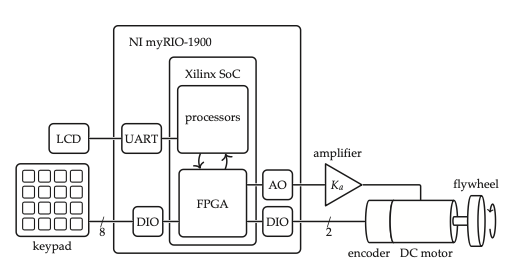
\includegraphics[width=.9\linewidth]{figures/Schema-Closed-Loop.png}
	\caption{Schematic diagram of the target closed-loop system \citep{Picone2024}.}
	\label{fig:SchemaClosedLoop}
\end{figure}

The objectives of this lab were:

\begin{enumerate}
	\item To implement a position control system for an inertia-dominated load
	\item To explore appropriate path planning
	\item To integrate the use of a standard MATLAB design tool into the application development system
\end{enumerate}

\section{Materials and Methods}

\subsection{Materials}
The materials used in this experiment were:
\begin{itemize}
	\item Windows 10 computer with myRIO support for C and Eclipse IDE.
	\item NI myRIO-1900
	\item Keypad
	\item Serial display
	\item PMDC motor
	\item Analog current amplifier
	\item DC power supply
	\item Quadrature encoder
	\item Flywheel
	\item MATLAB (version R2026a Update 3 used)
\end{itemize}

\subsection{PID Controller Design in MATLAB}
MATLAB was used as the primary design environment to tune a proportional-integral-derivative (PID) controller suitable for the plant dynamics in this lab. The controller structure used for design and analysis is shown in Figure~\ref{fig:PIDControlBlockDiagram}.
For context, Figure~\ref{fig:ControlBlockDiagram} shows the control architecture from the previous lab (Lab 7), which was based on PI velocity control. 

Comparing the two diagrams highlights the key change in this work: the PID/PIDF design introduces derivative action (with filtering) to improve transient shaping and robustness to measurement noise relative to the earlier PI-only formulation.

\begin{figure}[htb]
	\centering
	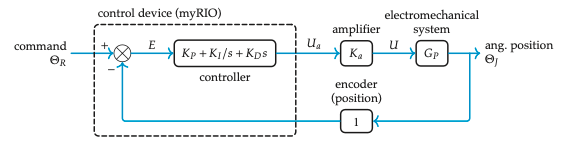
\includegraphics[width=.85\linewidth]{figures/PID_Control_Block_Diagram.png}
	\caption{PID controller block diagram used for controller design \citep{Picone2024}.}
	\label{fig:PIDControlBlockDiagram}
\end{figure}

\begin{figure}[htb]
	\centering
	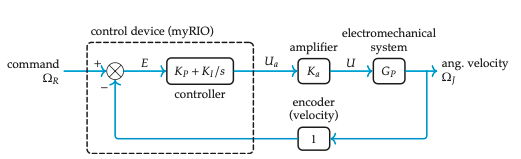
\includegraphics[width=.95\linewidth]{figures/Control-Block-Diagram.png}
	\caption{Control block diagram for the Lab 7 PI velocity-control system \citep{Picone2024}.}
	\label{fig:ControlBlockDiagram}
\end{figure}

\subsection{MATLAB Scripts}
Two MATLAB scripts were developed for this portion of the lab: one for PID-family controller synthesis and one for performance evaluation against reference and model-based responses.

\subsubsection{PID Controller Script}
The first script was used to tune a PIDF compensator with MATLAB's Control System Toolbox using \texttt{pidtune()}. The design target was closed-loop reference tracking with an approximate control bandwidth of $10\,\text{Hz}$. A derivative-filtered PID (PIDF) form was selected to improve noise robustness by rolling off the high-frequency gain of the derivative action.

After obtaining the continuous-time controller model, the script converted it to a discrete-time implementation using \texttt{tf()}, \texttt{c2d()}, and \texttt{tfdata()} with sampling time $T = 0.005\,\text{s}$. The resulting discrete transfer function was then decomposed into second-order sections with \texttt{tf2sos()} to produce biquad realizations. Finally, \texttt{sos2header()} (Appendix E.1) exported those biquad coefficients to the C header file \texttt{myPIDF.h}, which was subsequently included by the program's \texttt{main()} routine.

\subsubsection{Performance Analysis Script}
The second script loaded the measured position-control response from \texttt{Lab8.mat} and compared it with two benchmarks: the ideal reference displacement trajectory and the response predicted by the dynamic model.

\section{Laboratory Exploration and Evaluation}

\subsection{Problem L8.1}
Write, test, and debug the program described in section L8.3.

\vspace{\baselineskip}

The program can be found at \url{https://github.com/juliansoh/ME477/blob/main/workspace/Julian_lab8/main.c}.

The program follows the same overall architecture used in Lab 7: a Main thread handled setup and user interaction through \texttt{ctable2()}, while a Timer thread handled interrupt-timed control execution and data logging. In this lab, the active controller definition was taken from the header generated by the MATLAB design script.

\paragraph{L8.3.1 Two Threads.}
\textbf{Main Thread.} The Main thread was responsible for initialization, thread setup, and operator interaction. Its flow was:
\begin{enumerate}
	\item Initialize table-editor variables.
	\item Initialize path-profile variables for ramp generation.
	\item Configure the timer IRQ source (consistent with Labs 6 and 7).
	\item Register and create the Timer thread, passing pointers to both the table data and the path profile through the thread-resource structure.
	\item Launch the table editor with three display-only fields:
	\begin{itemize}
		\item \texttt{P\_ref}: revs
		\item \texttt{P\_act}: revs
		\item \texttt{VDAout}: mV
	\end{itemize}
	\item On table-editor exit, clear the Timer-thread ready flag and wait for clean thread termination.
\end{enumerate}

A representative resource structure was:
\begin{lstlisting}[language=C]
typedef struct {
  NiFpga_IrqContext irqContext; // context
  table *a_table;               // table
  seg *profile;                 // profile
  int nseg;                     // no. of segs
  NiFpga_Bool irqThreadRdy;     // ready flag
} ThreadResource;
\end{lstlisting}

\textbf{Timer Thread.} The Timer thread called the ISR-side logic each sample period. At thread start, shorthand pointers were created for table channels and ramp data, for example:
\begin{lstlisting}[language=C]
double *pref  = &((threadResource->a_table + 0)->value);
double *pact  = &((threadResource->a_table + 1)->value);
double *VDAmV = &((threadResource->a_table + 2)->value);
seg *mySegs = threadResource->profile;
int nseg = threadResource->nseg;
\end{lstlisting}

The thread ran in an IRQ-paced loop and exited only when its ready flag was cleared. Before entering the loop, it initialized analog I/O, forced the motor command to zero with \texttt{Aio\_Write()}, and configured the encoder counter interface.

At each interrupt cycle, it performed the following:
\begin{enumerate}
	\item Arm the next interval by waiting on IRQ assertion, writing the Timer Write Register, and writing \texttt{TRUE} to the Timer Set Time Register.
	\item Call \texttt{Sramps()} to compute the current reference position $\Theta_R$.
	\item Call \texttt{pos()} to measure motor position $\Theta_J$.
	\item Compute control error as $e = \Theta_R - \Theta_J$.
	\item Call \texttt{cascade()} with the PIDF filter to compute control voltage, then clamp the command to $[-10.0, +10.0]$ V.
	\item Write the command to DAC channel AOC0 via \texttt{Aio\_Write()}.
	\item Update table display values to reflect current controller state.
	\item Log current-sample data for later analysis.
\end{enumerate}

\paragraph{L8.4 Functions.}
Three functions were required inside the ISR loop:
\begin{itemize}
	\item \texttt{cascade()}: reused the Lab 6 biquad difference-equation implementation (double-precision arithmetic throughout). For this application, one biquad section was used.
	\item \texttt{pos()}: read the encoder counter and returned displacement as \texttt{double} in BDI (encoder counts), referenced to the first recorded position.
	\item \texttt{Sramps()}: generated the reference trajectory $\Theta_R$ from a segment list, advancing one step per control cycle and repeating the full path continuously.
\end{itemize}

The path profile was initialized in \texttt{main()} and passed to the Timer thread using pointers in the shared resource structure. Access to the segment type required:
\begin{lstlisting}[language=C]
#include "sramps.h"

typedef struct {
  double xfa; // position
  double v;   // velocity limit
  double a;   // acceleration limit
  double d;   // dwell time (s)
} seg;
\end{lstlisting}

For Lab 8 testing, the profile used eight ramp segments:
\begin{lstlisting}[language=C]
double vmax = 50.0;
double amax = 20.0;
double dwell = 1.0;

seg mySegs[8] = {
  {10.125, vmax, amax, dwell},
  {20.250, vmax, amax, dwell},
  {30.375, vmax, amax, dwell},
  {40.500, vmax, amax, dwell},
  {30.625, vmax, amax, dwell},
  {20.750, vmax, amax, dwell},
  {10.875, vmax, amax, dwell},
  { 0.000, vmax, amax, dwell}
};
int nseg = 8;
\end{lstlisting}

This sequence produced four equal upward ramps (each 10.125 rev), followed by four downward ramps that returned the shaft to its starting position. All segments shared the same velocity and acceleration limits, with a 1 s dwell at each endpoint before progressing to the next segment.

The collected data were then opened in MATLAB from the \texttt{Lab8.mat} file, and the resulting plot is shown in Figure~\ref{fig:Lab8DataPlot}.

\begin{figure}[h]
\centering
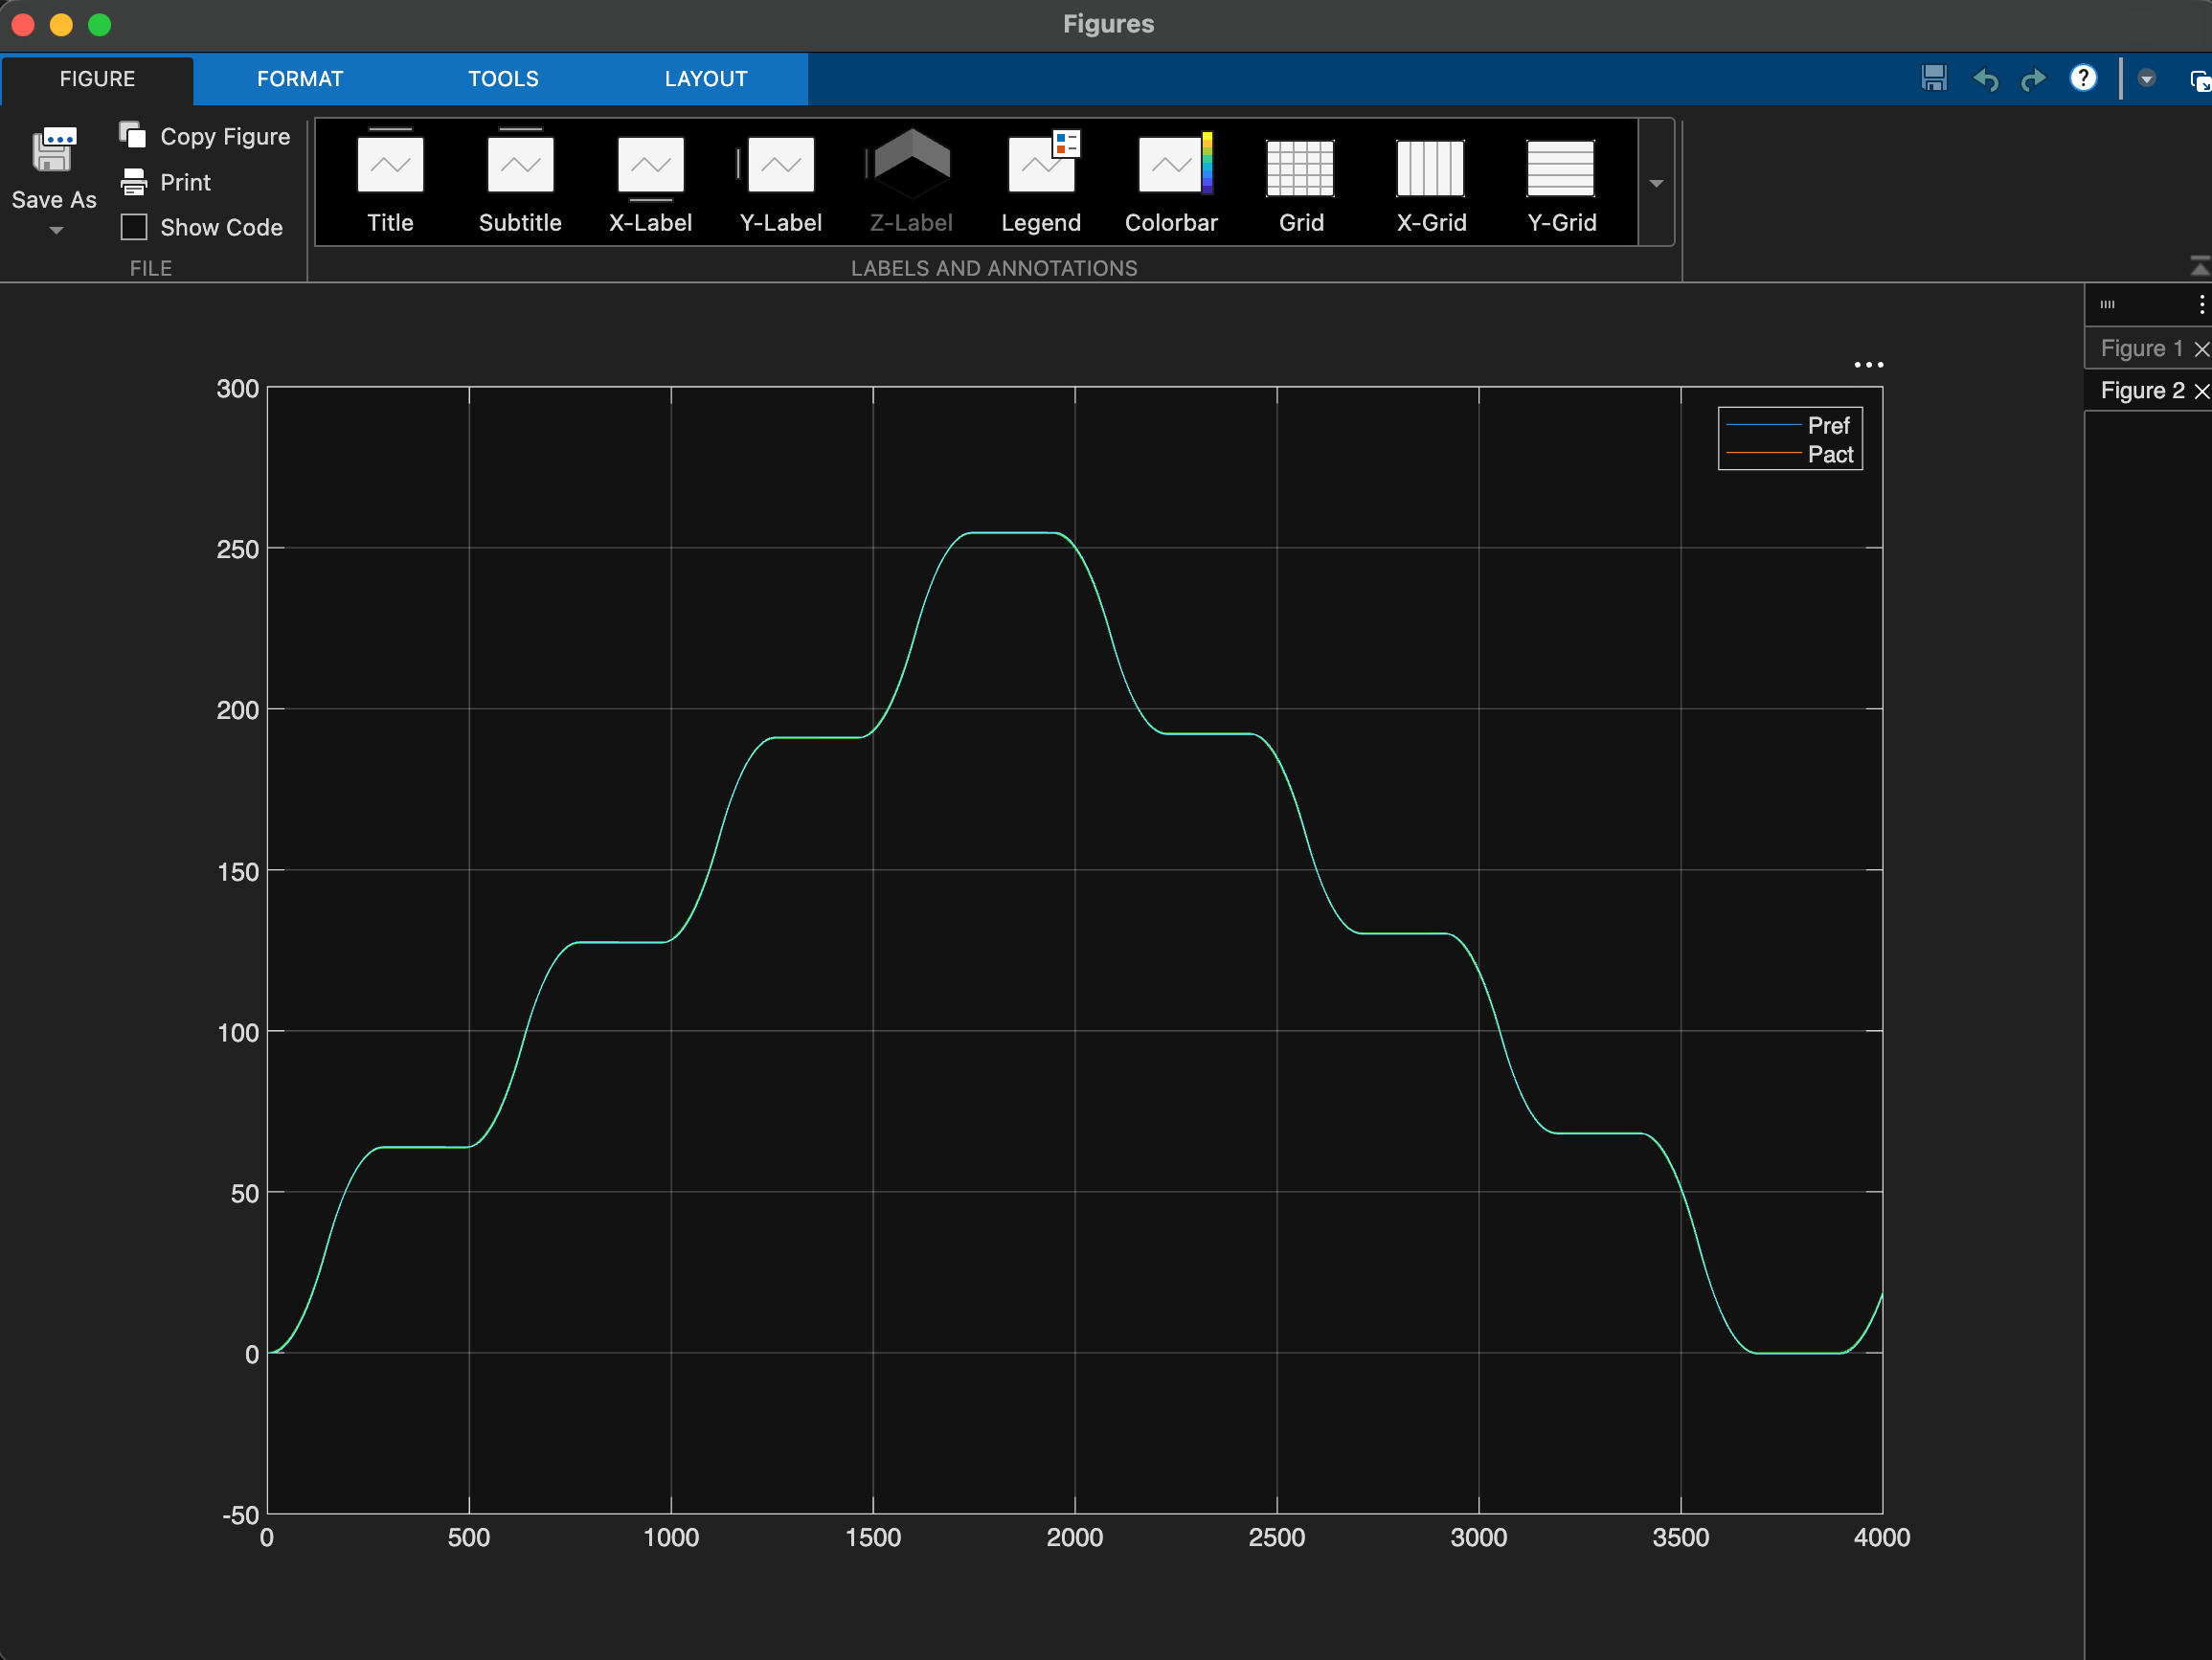
\includegraphics[width=0.95\columnwidth]{figures/Plot_Of_Lab8_Data.png}
\caption{MATLAB plot generated from the collected data stored in \texttt{Lab8.mat}.}
\label{fig:Lab8DataPlot}
\end{figure}

\subsection{Problem L8.2}
Write a MATLAB script (not the one in which you designed
the controller) to analyze the result of running the program that you wrote in lab
problem L8.1. It should do the following.
\begin{enumerate}
\item Load the experimental results from the Lab8.mat file.
\item Define a discrete version of the motor/load plant transfer from lab exercise 7.
Consider using c2d().
\item Form the discrete controller from the values in the PIDF array in Lab8.mat.
\item Form the closed-loop system models relating the reference position $\Theta_R$ input to
the position $\Theta_J$ and torque $T$ outputs:
\[
\frac{\Theta_J(z)}{\Theta_R(z)} = G_1(z), \qquad \frac{T(z)}{\Theta_R(z)} = G_2(z).
\]
\item Using lsim(), simulate the system to find the theoretical responses for both the
position $\Theta_J(t)$ and the torque $T(t)$ to the reference position $\Theta_R(t)$ array that you
stored in Lab8.mat.
\item In a single MATLAB figure, plot the results in three subplot()s versus time, as
follows:
\begin{enumerate}
\item Reference position, theoretical position, and experimental position.
\item Experimental error (reference-experimental position) and theoretical
error (reference-theoretical position).
\item Theoretical and experimental torque.
\end{enumerate}
\end{enumerate}

\subsection{Problem L7.3}
Write, test, and debug the program described in Section L7.2. For debugging purposes, use the base set of parameters.

The PI motor velocity controller described in Section L7.2 was implemented in C and tested on the myRIO platform using the base controller gains $K_P = 0.104\;\text{V\,s/rad}$ and $K_I = 2.07\;\text{V/rad}$. Several debugging steps were required to verify proper operation of the velocity measurement, controller calculations, and actuator output. After correcting implementation issues, the controller successfully regulated motor speed. During testing, the measured velocity converged to approximately the commanded speed and the control output remained bounded. As shown in Figure~\ref{fig:steady_state_evidence} (Figure 3), the final implementation exhibited stable closed-loop operation and was used for the remaining laboratory exercises.

A video of this steady-state experiment could be found at \url{https://github.com/juliansoh/ME477/blob/main/Reports/Lab7/videos/Steady-state.mp4}.

The program implementation is available at \url{https://github.com/juliansoh/ME477/blob/main/workspace/Julian_lab7/main.c}.

\section{Author Contributions}

There was only one author for this report and lab.



%%% References -------------------------

\bibliographystyle{plainnat}
\bibliography{report}

%%% Appendices -------------------------

\end{document}  